\documentclass[letterpaper,12pt]{article}
\usepackage[utf8]{inputenc}
\usepackage{fullpage}
\usepackage{courier}
\usepackage[margin=0.75in]{geometry}
\usepackage{listings}
\usepackage{color}
\usepackage{graphicx}
\usepackage[width=4in]{caption}
\usepackage{hyphenat}

% Format a sectionless paragraph
\newcommand*\unparagraph{
	\par
	\nopagebreak
	\vskip3.25ex plus1ex minus.2ex
	\noindent
}

% define extra colors
\definecolor{dkgreen}{rgb}{0,0.6,0}
\definecolor{purple}{RGB}{159,0,197}

% define the code listing format
\lstset{language=C++,
	basicstyle=\ttfamily,
	backgroundcolor=\color{white},
	showspaces=false,
	showstringspaces=false,
	frame=none,
	tabsize=3,
	keywordstyle=\color{purple},
	commentstyle=\color{dkgreen},
	stringstyle=\color{blue},
	escapeinside={\%*}{*)}
}

% define the title/header
\title{\Large CS 1428\\Lab 10 Sections L19 and L06} 
\author{Jared Wallace}
\date{}

\begin{document}

\maketitle

\section*{Functions (cont.)}
\begin{enumerate}
	\item Write a function named timesTen.  The function should have an integer parameter named number.  When timesTen is called, it should display the product of number and 10.  (Note:  Just write the function definition.  Do not write a complete program.)
		\vspace{20mm}
	\item Write the function prototype for the timesTen function that you wrote in Question 1.
		\vspace{15mm}
	\item A program contains the following function:
	\begin{lstlisting}[basicstyle=\footnotesize\ttfamily]
int  cube(int  num)
{
	return  num  *  num  *  num;
}
		\end{lstlisting}
		Write a statement that passes the value 4 to this function and assigns its return value to the variable result.  Assume that result has been declared.
		\vspace{20mm}
	\item The following program asks the user to enter two numbers. What is the output of the program after the user enters 12 then 14 when prompted?
	
	\begin{lstlisting}[basicstyle=\footnotesize\ttfamily]
#include <iostream>
using namespace std;

void func1(int &, int &);
void func2(int &, int &, int &);
void func3(int, int, int);

int main()
{
	int x = 0, y = 0, z = 0;

	cout << x << " " << y << " " << z << endl;
	func1(x, y);
	cout << x << " " << y << " " << z << endl;
	func2(x, y, z);
	cout << x << " " << y << " " << z << endl;
	func3(x, y, z);
	cout << x << " " << y << " " << z << endl;
	return 0;
}

void func1(int &a, int &b)
{
		cout << "Enter two numbers: ";
			cin >> a >> b; 
}

void func2(int &a, int &b, int &c)
{
	b++;
	c--;
	a = b + c;
}

void func3(int a, int b, int c)
{
	a = b - c;
}
	\end{lstlisting}

	\vspace{20mm}

	\item Write a program (lab10\_01.cpp) that calculates the gross pay of an employee. Your program should: 
		\begin{enumerate}
         \item have the following \textbf{global} constants declared
				\begin{enumerate}
					\item PAY\_RATE = 20.55
					\item BASE\_HOURS = 30.0
					\item OT\_MULTIPLIER = 1.5
				\end{enumerate}
			\item Ask the user to enter the number of hours worked (Note:  Be sure to validate the hour entered by the user. Do not accept negative values for hours. )
         \item Get the amount of base pay (using a function)
         \item Get overtime pay if any (using a function)
			\item Display the employee's base pay, overtime pay, and total pay
      \end{enumerate}
\textbf{To determine the base pay:}
If the hours worked is greater than the base hours, then base pay equals base hours times the pay rate. Otherwise, base pay equals the hours worked times the pay rate.


\textbf{To determine the overtime pay}
If the hours worked is greater than the base hours, then overtime pay equals hours worked minus base hours, times the pay rate multiplied by the overtime multiplier. Otherwise, overtime pay equals zero.

For example: If the hours worked are 35, then the base pay is 30 * 20.55, and the overtime pay is 5 * 20.55 * 1.5.
\end{enumerate}
\vspace{20mm}

% Don't forget the submission instructions!
\unparagraph{} \textbf{Upload your source code lab10.cpp and attach a print out to this worksheet.}

\vspace{20mm}

% Comic at the bottom
\begin{figure}[ht!]
	\centering
	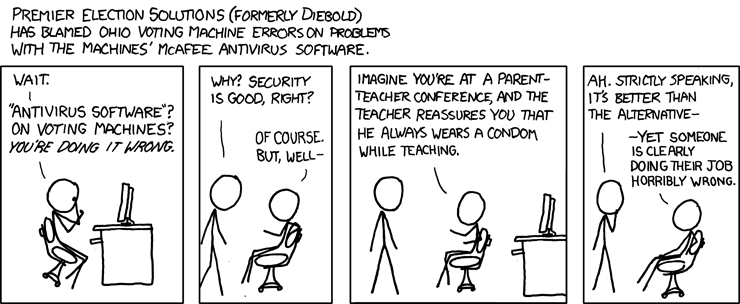
\includegraphics[width=6in]{voting_machines.png}
	\caption*{And thats *another* crypto conference I've been kicked out of. C'mon, it's a great analogy!}
\end{figure}

\end{document}
